\section{Tank Model - SMA (model ID: 38)}
The Tank Model (fig.~\ref{fig:38_schematic}) is originally developed for use in constantly saturated soils in Japan \citep{Sugawara1979}. This alternative Tank model - SMA (soil moisture accounting) version was developed for regions that are not continuously saturated \citep{Sugawara1995}. This model is identical to the original tank model, but has an increased depth in the first store to represent primary soil moisture, and adds a new store to represent secondary soil moisture. It has 5 stores and 16 parameters ($sm_1$, $sm_2$, $k_1$, $k_2$, $A_0$, $A_1$, $A_2$, $t_1$, $t_2$, $B_0$, $B_1$, $t_3$, $C_0$, $C_1$, $t_4$ and $D_1$). The model aims to represent:

\begin{itemizecompact}
\item Runoff on increasing time scales with depth;
\item Soil moisture storage;
\item capillary rise to replenish soil moisture.
\end{itemizecompact}

\subsection{MARRMoT model name}
m\_38\_tank2\_16p\_5s \\

% Equations
\subsection{Model equations}

% Model layout figure
{ 																	% This ensures it doesn't warp text further down
\begin{wrapfigure}{l}{6cm}
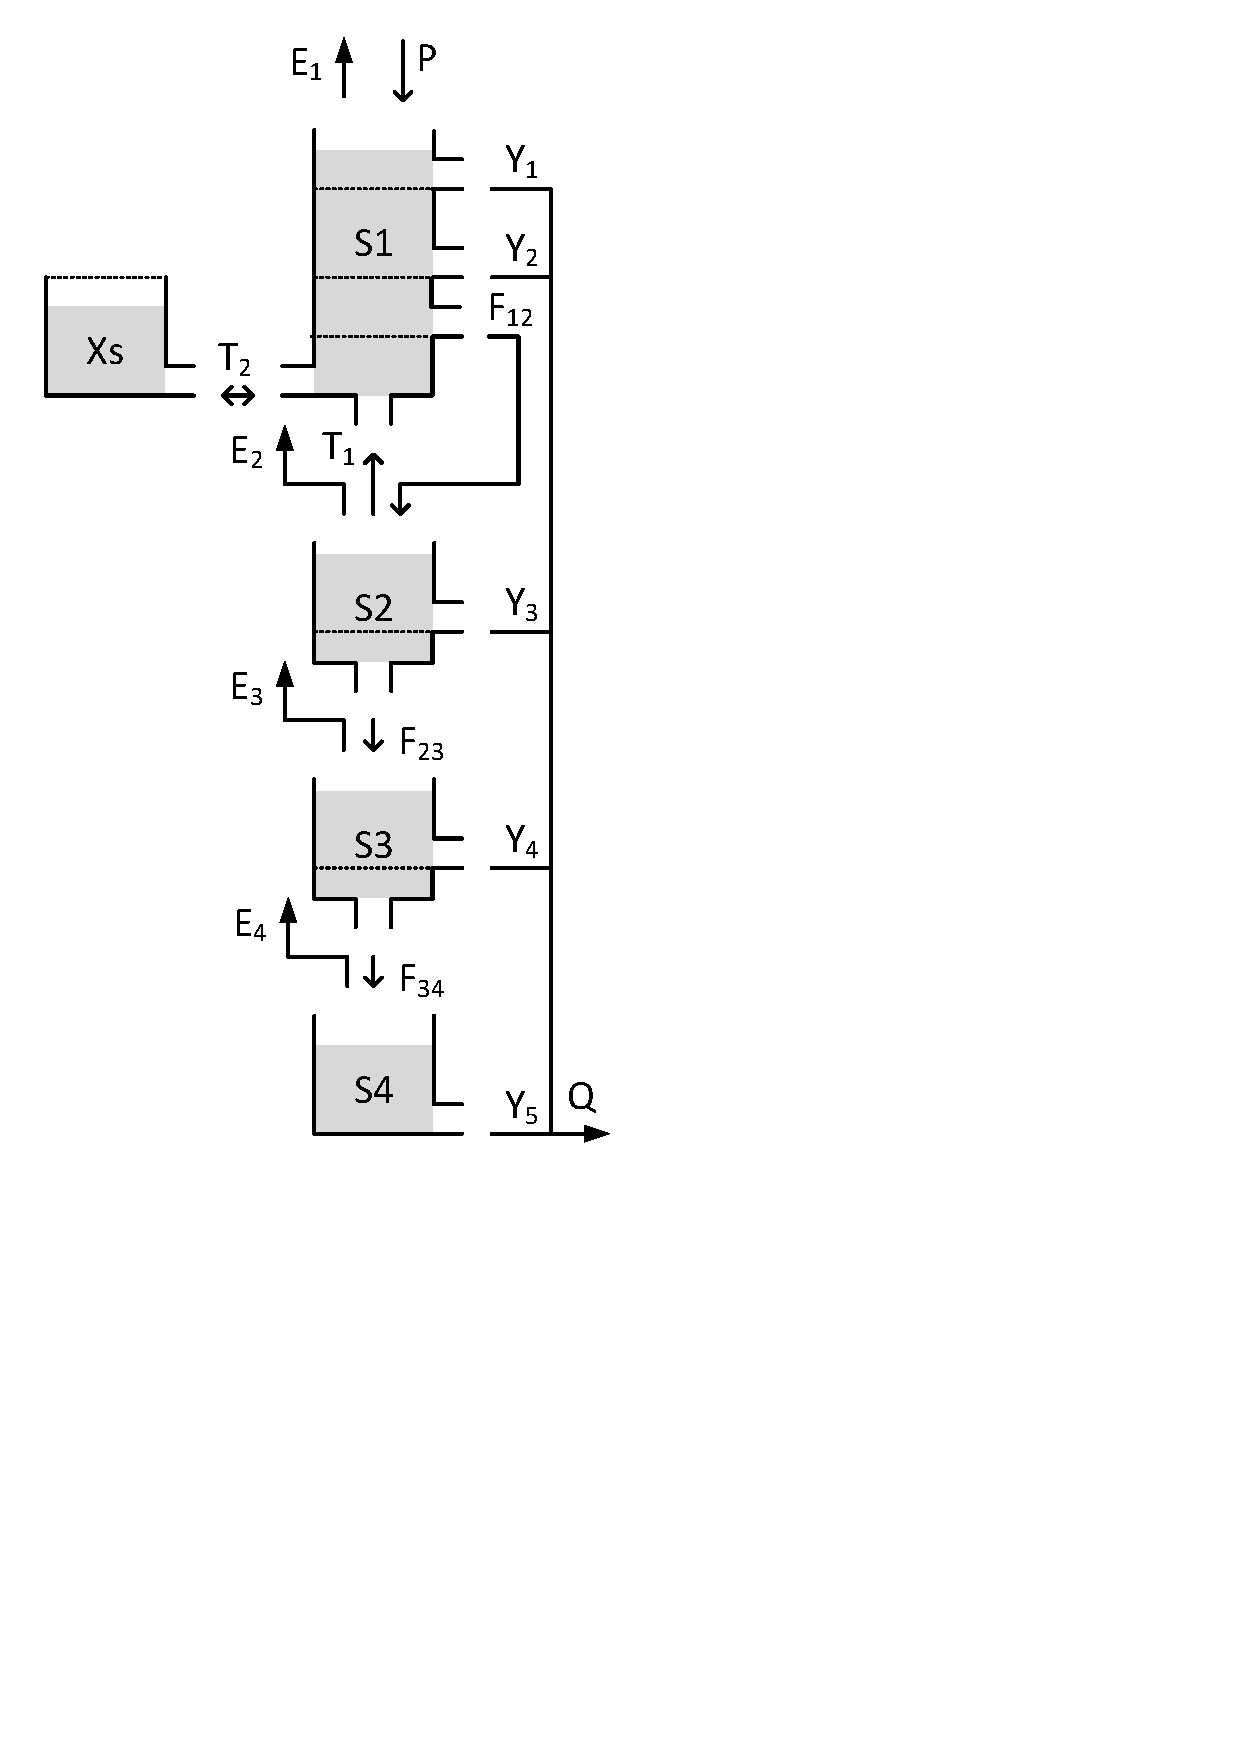
\includegraphics[trim=1cm 10cm 7cm 1cm,width=7cm,keepaspectratio]{./AppA_files/38_schematic.pdf}
\caption{Structure of the Tank Model - SMA} \label{fig:38_schematic}
\end{wrapfigure}

\begin{align}
	\frac{dS_1}{dt} &= P+T_1-T_2-E_1-F_{12}-Y_2-Y_1 \\
	T_1 &= k_1\left(1-\frac{S_1}{sm_1}\right), \text{if } S_1 < sm_1\\
	T_2 &= k_2\left(\frac{min(S_1,sm_1)}{sm_1}-\frac{X_s}{sm_2}\right) \\
	E_1 &= \begin{cases}
		Ep, &\text{if } S_1 > 0 \\
		0, & \text{otherwise} \\
	\end{cases} \\
	F_{12} &= \begin{cases}
		A_0*(S_1-sm_1), & \text{if } S_1 > sm_1 \\
		0, & \text{otherwise}
	\end{cases}\\
	Y_2 &= 
	\begin{cases}
		A_2*(S_1-t_2), & \text{if } S_1 > t_2 \\
		0, & \text{otherwise}
	\end{cases}\\
	Y_1 &= 
	\begin{cases}
		A_1*(S_1-t_1), & \text{if } S_1 > t_1 \\
		0, & \text{otherwise}\\
	\end{cases}
\end{align}

Where $S_1$ [mm] is the current storage in the upper zone, refilled by precipitation $P$ 

} % end of wrap figure

\noindent$[mm/d]$ and drained by evaporation $E_1$ $[mm/d]$, drainage $F_{12}$ $[mm/d]$ and surface runoff $Y_1$ $[mm/d]$ and $Y_2$ $[mm/d]$. If $S_1$ is below the soil moisture threshold $sm_1$ [mm], capillary rise $T_1$  $[mm/d]$ from store $S_2$ can occur. Capillary rise has a base rate $k_1$  $[mm/d]$ and decreases linearly as soil moisture $S_1$ nears $sm_1$. This store is connected to the secondary soil moisture store $X_s$ through transfer flux $T_2$  $[mm/d]$. This flux can work in either direction, based on a base rate $k_2$ [mm/d], the current storages $S_1$ [mm] and $X_s$ [mm] and the maximum soil moistures storages $sm_1$ [mm] and $sm_2$ [mm]. Evaporation $E_1$ occurs at the potential rate $E_p$ $[mm/d]$ if water is available. Drainage to the intermediate layer has a linear relationship with storage through time scale parameter $A_0$ $[d^{-1}]$. Surface runoff $Y_2$ and $Y_1$ occur when $S_1$ is above thresholds $t_2$ [mm] and $t_1$ [mm] respectively. Both are linear relationships through time parameters $A_2$ $[d^{-1}]$ and $A_1$ $[d^{-1}]$ respectively.

\begin{align}
	\frac{dX_s}{dt} &= T_2
\end{align}

Where $X_s$ [mm] is the current storage in the secondary soil moisture zone. This zone has a maximum capacity $sm_2$ [mm], used in the calculation of $T_2$. $T_2$ can be both positive and negative.

\begin{align}
	\frac{dS_2}{dt} &= F_{12}-E_2-T_1-F_{23}-Y_3\\
	E_2 &= \begin{cases}
		Ep, &\text{if } S_1 = 0 ~\&~ S_2 > 0\\
		0, & \text{otherwise} \\
	\end{cases} \\
	F_{23} &= B_0*S_2\\
	Y_3 &= 
	\begin{cases}
		B_1*(S_2-t_3), & \text{if } S_2 > t_3 \\
		0, & \text{otherwise}
	\end{cases}
\end{align}

Where $S_2$ [mm] is the current storage in the intermediate zone, refilled by drainage $F_{12}$ from the upper zone and drained by evaporation $E_2$ $[mm/d]$, drainage $F_{23}$ $[mm/d]$ and intermediate discharge $Y_3$ $[mm/d]$. $E_2$ occurs at the potential rate $E_p$ if water is available and the upper zone is empty. Drainage to the third layer $F_{23}$ has a linear relationship with storage through time scale parameter $B_0$ $[d^{-1}]$. Intermediate runoff $Y_3$ occurs when $S_2$ is above threshold $t_3$ [mm] and has a linear relationship with storage through time scale parameter $B_1$ $[d^{-1}]$.

\begin{align}
	\frac{dS_3}{dt} &= F_{23}-E_3-F_{34}-Y_4\\
	E_3 &= \begin{cases}
		Ep, &\text{if } S_1 = 0 ~\&~ S_2 = 0 ~\&~ S_3 > 0\\
		0, & \text{otherwise} \\
	\end{cases} \\
	F_{34} &= C_0*S_3\\
	Y_4 &= 
	\begin{cases}
		C_1*(S_3-t_4), & \text{if } S_3 > t_4 \\
		0, & \text{otherwise}
	\end{cases}
\end{align}

Where $S_3$ [mm] is the current storage in the sub-base zone, refilled by drainage $F_{23}$ from the intermediate zone and drained by evaporation $E_3$ $[mm/d]$, drainage $F_{34}$ $[mm/d]$ and sub-base discharge $Y_4$ $[mm/d]$. $E_3$ occurs at the potential rate $E_p$ if water is available and the upper zones are empty. Drainage to the fourth layer $F_{34}$ has a linear relationship with storage through time scale parameter $C_0$ $[d^{-1}]$. Sub-base runoff $Y_4$ occurs when $S_3$ is above threshold $t_4$ [mm] and has a linear relationship with storage through time scale parameter $C_1$ $[d^{-1}]$.

\begin{align}
	\frac{dS_4}{dt} &= F_{34}-E_4-Y_5\\
	E_4 &= \begin{cases}
		Ep, &\text{if } S_1 = 0 ~\&~ S_2 = 0 ~\&~ S_3 = 0 ~\&~ S_4 > 0\\
		0, & \text{otherwise} \\
	\end{cases} \\
	Y_5 &= D_1*S_4
\end{align}

Where $S_4$ [mm] is the current storage in the base layer, refilled by drainage $F_{34}$ from the sub-base zone and drained by evaporation $E_4$ $[mm/d]$ and baseflow $Y_5$ $[mm/d]$. $E_4$ occurs at the potential rate $E_p$ if water is available and the upper zones are empty. Baseflow $Y_5$ has a linear relationship with storage through time scale parameter $D_1$ $[d^{-1}]$. Total runoff:

\begin{align}
	Q_t &= Y_1+Y_2+Y_3+Y_4+Y_5
\end{align}

\newpage
\subsection{Parameter overview}
% Table generated by Excel2LaTeX from sheet 'Sheet1'
\begin{table}[htbp]
  \centering
    \begin{tabular}{lll}
    \toprule
    Parameter & Unit  & Description \\
    \midrule
    $sm_1$ & $mm$  & Soil moisture threshold for capillary rise \\
    $sm_2$ & $mm$  & Maximum soil mositure storage \\
    $k_1$ & $mm~d^{-1}$ & Base capillary rise rate \\
    $k_2$ & $mm~d^{-1}$ & Base soil moisture exchange rate \\
    $A_0$ & $d^{-1}$ & Runoff coefficient \\
    $A_1$ & $d^{-1}$ & Runoff coefficient \\
    $A_2$ & $d^{-1}$ & Runoff coefficient \\
    $t_1$ & $mm$  & Threshold for runoff generation \\
    $t_2$ & $mm$  & Threshold for runoff generation \\
    $B_0$ & $d^{-1}$ & Runoff coefficient \\
    $B_1$ & $d^{-1}$ & Runoff coefficient \\
    $t_3$ & $mm$  & Threshold for runoff generation \\
    $C_0$ & $d^{-1}$ & Runoff coefficient \\
    $C_1$ & $d^{-1}$ & Runoff coefficient \\
    $t_4$ & $mm$  & Threshold for runoff generation \\
    $D_1$ & $d^{-1}$ & Runoff coefficient \\
    \bottomrule
    \end{tabular}%
  \label{tab:addlabel}%
\end{table}%
